\documentclass[tikz,border=10pt]{standalone}
\begin{document}
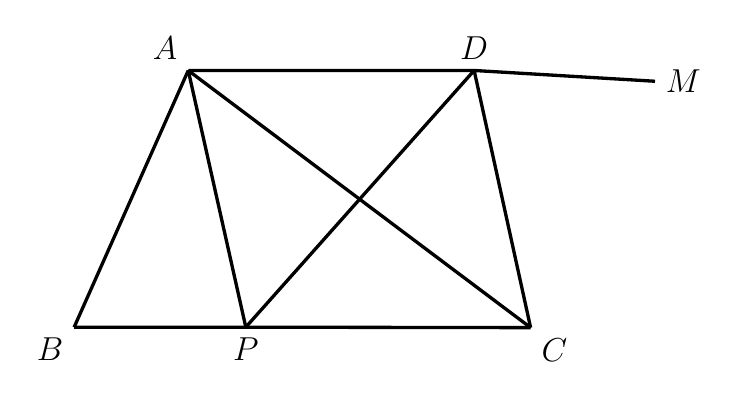
\begin{tikzpicture}[line width=1.2pt, line join=round, font=\fontsize{12}{14.4}\selectfont]
\coordinate (A) at (-2.066,1.637);
\coordinate (B) at (-3.515,-1.623);
\coordinate (C) at (2.282,-1.629);
\coordinate (D) at (1.565,1.637);
\coordinate (M) at (3.862,1.500);
\coordinate (P) at (-1.335,-1.623);

  

  
  \draw (B) -- (P) -- (C);

  
  \draw (A) -- (B);
  \draw (D) -- (C);

  
  \draw (A) -- (P);
  \draw (A) -- (C);
  \draw (D) -- (P);

  
  \draw (A) -- (D) -- (M);

  
  \node[above left] at (A) {$A$};
  \node[above] at (D) {$D$};
  \node[below left] at (B) {$B$};
  \node[below] at (P) {$P$};
  \node[below right] at (C) {$C$};
  \node[right] at (M) {$M$};
\end{tikzpicture}
\end{document}